\documentclass[12pt, a4paper]{article}
\usepackage[utf8]{inputenc}
\usepackage[czech]{babel}
\usepackage[T1]{fontenc}
\usepackage{graphicx}
\usepackage{amsmath, amssymb, amsthm}
\usepackage[margin=2.5cm]{geometry}
\usepackage{url}
\usepackage{float}
\begin{document}

\begin{titlepage}
    \begin{center}
        {\large {Přírodovědecká fakulta}} \\
        \vspace{0.2cm}
        {\large Univerzita Karlova}
        
        \vspace{1.5cm}
        
\includegraphics[width=0.5\linewidth]{img/PrFUK_strom_digital_cerna.png} 
        \vfill{}
        
        {\huge\bfseries Hodnocení kartografických zobrazení s využitím variačních kritérií} \\
        \vspace{0.5cm}
        {\large {Matematická kartografie}} \\
        \vfill
        
        \begin{center}
            \large Teodor Sorokáč \\
        \end{center}
        \vfill{}

        \begin{center}
            \ 2. N-GKDPZ \\
            \ Praha 2026
        \end{center}
        
    \end{center}
\end{titlepage}

\section{Zadání}

\vspace{5mm}
\subsection*{\textbf{Úloha č. 4: Hodnocení kartografických zobrazení s využitím variačních kritérií}}

\vspace{3mm}
Na základě globálních variačních kritérií proveďte zhodnocení níže uvedených zobrazení a rozhodněte o jejich vhodnosti (či nevhodnosti) pro mapy velkých územních celků.
\vspace{3mm}

\noindent Přehled lokálních variačních kritérií v bodě $P=[u,v]$:
\begin{itemize}
    \item \textbf{Airyho kritérium (komplexní kritérium):}
\end{itemize}
\[
\begin{aligned}
h^{2}(u,v) &= \frac{(a-1)^{2}+(b-1)^{2}}{2}, \\
h^{2}(u,v) &= \frac{|a-1|+|b-1|}{2}+\frac{a}{b}-1.
\end{aligned}
\]

\vspace{3mm}
\noindent Pro kartografická zobrazení volená v normální poloze spočtěte hodnoty lokálních kritérií $h^{2}(u,v)$ v uzlových bodech geografické sítě pokrývajících zadané území a jeho nejbližší okolí s kroky $\Delta u = \Delta v = 10^{\circ}$ (resp. s polovičním krokem, je-li třeba). Území by mělo být pokryto alespoň 30 uzlovými body. Při výpočtu využijte osové symetrie geografické sítě dle rovníku či základního poledníku.
\vspace{3mm}

\noindent Z hodnot lokálních kritérií $h^{2}(u,v)$ v uzlových bodech určete pro každé kartografické zobrazení hodnoty globálních kritérií. Globální variační kritérium $H^{2}$ nahraďte diskrétními vztahy, uvažujte neváženou i váženou variantu, kde váha je definována jako $p_{i} = \cos u_{i}$:
\[
H^{2} = \frac{1}{(u_{2}-u_{1})(v_{2}-v_{1})} \int_{u_{1}}^{u_{2}} \int_{v_{1}}^{v_{2}} h^{2} \cos u \, \mathrm{d}u \, \mathrm{d}v,
\]
\[
H_{1}^{2} = \frac{1}{n} \sum_{i=1}^{n} h^{2}(u_{i},v_{i}), \quad H_{2}^{2} = \frac{\sum_{i=1}^{n} p_{i} h^{2}(u_{i},v_{i})}{\sum_{i=1}^{n} p_{i}}.
\]

\vspace{3mm}
\noindent \textbf{Přehled analyzovaných kartografických zobrazení:}
\begin{itemize}
    \item Bonneovo,
    \item Mercator-Sansonovo,
    \item Eckertovo V.,
    \item Winkel-Tripel,
    \item Hammer-Aitoffovo.
\end{itemize}

\vspace{3mm}
\noindent V uzlových bodech geografické sítě vypočtěte měřítkové číslo $M(u,v)$ mapy jako funkci polohy:
\[
M(u,v) = \frac{M}{\max_{A} m(u,v,A)} = \frac{M}{a(u,v)}
\]

\noindent vygenerujte také jeho izočáry. Výchozí hodnotu měřítkového čísla volte pro formát A4, pro mapu planisféry např. $M = 100\,000\,000$. Výpočty proveďte na jednotkové kouli, zeměpisnou šířku $u_{0}$ nezkreslené rovnoběžky volte tak, aby procházela (stejně jako základní poledník $v_{0}$) středem zobrazovaného území.
\vspace{3mm}

\noindent V přehledných tabulkách uveďte hodnoty globálních kritérií a rozhodněte, které z kartografických zobrazení je nejvhodnější pro znázornění zvoleného územního celku. V závěru také zhodnoťte, jaké variační kritérium dle Vašeho názoru lépe vystihuje vlastnosti kartografického zobrazení. Výpočty proveďte s využitím programu Proj4 či skriptu v programu MATLAB.

\vspace{5mm}
\noindent \textbf{Územní celky:} \\
Kromě níže navržených územních celků je možné navrhnout i vlastní celky.

\vspace{3mm}
\begin{center}
\begin{tabular}{rlrl}
1. & Evropa & 12. & státy sdružení ASEAN \\
2. & státy EU & 13. & Austrálie a Oceánie \\
3. & Afrika, Středozemní moře, Madagaskar & 14. & Indický oceán \\
4. & Rusko & 15. & Atlantský oceán \\
5. & Čína, Indie, Mongolsko & 16. & Jižní Amerika \\
6. & státy Arabské ligy & 17. & státy Varšavské smlouvy \\
7. & Kanada & 18. & Sibiř, Aljaška \\
8. & USA, Mexiko & 19. & asijští tygři \\
9. & Tichý oceán & 20. & země NAFTA \\
10. & arabsky hovořící země (Asie) & 21. & skandinávské státy, Grónsko \\
11. & země bývalého SSSR (bez Ruska) & 22. & účastníci I. / II. světové války \\
\end{tabular}
\end{center}

\vspace{1cm}
\subsection*{\textbf{Hodnocení:}}

\begin{center}
\resizebox{\textwidth}{!}{
\begin{tabular}{|l|c|}
\hline
\textbf{Krok}                                                                                   & \textbf{Hodnocení} \\ [0.5ex]  \hline\hline
\rule{0pt}{3ex} Hodnocení kartograf. zobrazení s využitím variačních kritérií.                 &  20b               \\ \hline
\rule{0pt}{3ex} Vážená varianta kritérií.                                                       &  +5b               \\ \hline
\rule{0pt}{3ex} Analýza velikosti kroků $\Delta u$ na hodnoty kritérií.                         &  +10b              \\ \hline
\rule{0pt}{3ex} Jaké procento území má zkreslení úhlů menší než 50\,\%.                         &  +10b              \\ \hline
\rule{0pt}{3ex} Jaké procento území má změnu $M$ menší než 50\,\%.                               &  +10b              \\ \hline
\rule{0pt}{3ex} Další hodnocené kartografické zobrazení (max. +3).                             &  +5b               \\ \hline
\rule{0pt}{3ex}\textbf{Max celkem:}                                                             & \textbf{70b}       \\ \hline
\end{tabular}
}
\end{center}
\vspace{5mm}




\newpage
\section{Popis a rozbor problému}
Pro účel zhodnocení kartografických zobrazení se využívají variační kritéria (lokální a globální kritéria), která všestraně ověří vhodnost zobrazení.

\subsection*{Lokální variační kritéria}
Pro výpočet variačního kritéria je nejprve nutné stanovit bod sítě, ve kterém se bude počítat $P = [u, v]$. Lokálním variačním kritériem je např. Airyho kritérium, které zohledňuje především vliv délkového zkreslení a je definováno vztahem:

\vspace{3mm}
\[
h^{2}(u,v) = \frac{(a-1)^{2}+(b-1)^{2}}{2}
\]

\vspace{3mm}
\noindent Komplexní kritérium navíc zohledňuje i úhlové zkreslení pomocí poměru poloos Tissotovy elipsy:
\vspace{3mm}

\[
h^{2}(u,v) = \frac{|a-1|+|b-1|}{2}+\frac{a}{b}-1
\]
\vspace{3mm}

\subsection*{Zkreslení úhlů a měřítka}
\noindent Pro zhodnocení úhlového zkreslení se v každém bodě sítě nejprve stanoví maximální úhlové zkreslení $\omega$ na základě poloos $a$ a $b$ pomocí vztahu:
\vspace{3mm}
\[
\omega = 2 \cdot \arcsin \left( \frac{|a - b|}{a + b} \right)
\]
\vspace{3mm}

\noindent Hodnota je převedena na stupně ($\omega_{\text{deg}}$) a poté se hodnotí všechny body sítě, splňující podmínku úhlového zkreslení menšího než $50^\circ$:

\vspace{3mm}
\[
\omega_{\text{deg}} < 50^\circ
\]

\vspace{3mm}
\noindent Pro spočítání odchylky od hlavního měřítka $M$ je zjišťováno zda dochází k deformaci v rozmezí $\pm 50\,\%$ od nezkresleného stavu ($a = 1$).
\vspace{3mm}

\[
0.5 \le a \le 1.5
\]

\vspace{3mm}
\noindent Výsledný podíl bodů sítě, které splňují podmínku, kde zkreslení nepřekročí hranici 50 \%, jsou vyhodnoceny jako vhodné pro zobrazení území v daném kartografickém zobrazení.

\subsection*{Globální variační kritéria}
Globální kritéria hodnotí celé zobrazované území. Pro výpočet je nutné sestavit síť bodů s krokem $\Delta u = \Delta v = 10^\circ$. Aritmetickým průměrem lokálních kriterií všech bodů vyjde nevážené globální variační kritérium:
\vspace{3mm}
\[
H_{1}^{2} = \frac{1}{n}\sum_{i=1}^{n}h^{2}(u_{i},v_{i})
\]
\vspace{3mm}
Vážené globální variační kritérium je počítáno se snahou odstranění vlivu odlehlých polárních oblastí. Vahou bodu je tedy funkce jeho zeměpisné šířky:
\vspace{3mm}
\[
H_{2}^{2} = \frac{\sum_{i=1}^{n}p_{i}h^{2}(u_{i},v_{i})}{\sum_{i=1}^{n}p_{i}}
\]


\newpage
\section{Zpracovaná kartografická zobrazení}
\vspace{3mm}
\subsection*{Bonneovo zobrazení}
\vspace{3mm}
Bonneovo zobrazení se řadí mezi nepravá kuželová zobrazení. Zobrazení je ekvivalentní, ekvidistantní podél rovnoběžek a má jednu nezkreslenou rovnoběžku $u_0$. Je vhodné pro mapování rozsáhlých územních celků rozkládajících se podél základního poledníku. Výpočet vychází z určení polárních souřadnic $\rho$ a $\epsilon$:

\vspace{3mm}
\[
\rho = R \cdot \cot u_0 + R(u_0 - u), \quad \epsilon = \frac{R \cdot v \cdot \cos u}{\rho}
\]

\vspace{3mm}
\noindent Polární souřadnice se převedou do pravoúhlých, kde souřadnice $x$ má tvar:
\vspace{3mm}
\[
x = \rho \cdot \sin \epsilon
\]
\vspace{3mm}
\noindent Souřadnice y je upravena posunutím počátku soustavy do průsečíku základního poledníku a nezkreslené rovnoběžky:
\vspace{3mm}

\[
y = R \cdot \cot u_0 - \rho \cdot \cos \epsilon
\]
\vspace{3mm}

\noindent Měřítko délek Bonneova zobrazení v poledníkovém směru je výjádřeno tímto vztahem:
\vspace{3mm}
\[
m_p = \sqrt{1 - (\epsilon - v \cdot \sin u)^2}
\]

\subsection*{Mercator-Sansonovo zobrazení}
\vspace{3mm}
Mercator-Sansonovo zobrazení patří mezi nepravá válcová zobrazení. Zobrazení je ekvivalentní a ekvidistantní podél rovnoběžek a má nezkreslený základní poledník. Obrazem poledníků jsou sinusoidy a obrazem rovnoběžek jsou rovnoběžné úsečky s konstantním rozestupem. Výpočet pravoúhlé souřadnice $x$ je dán vztahem:

\vspace{3mm}
\[
x = R \cdot v \cdot \cos u
\]
\vspace{3mm}

\noindent Souřadnice $y$ závisí lineárně pouze na zeměpisné šířce daného bodu:

\vspace{3mm}
\[
y = R \cdot u
\]
\vspace{3mm}

\noindent Měřítko délek v poledníkovém směru $m_p$ se určí ze vztahu:

\vspace{3mm}
\[
m_p = \sqrt{1 + v^2 \cdot \sin^2 u}
\]

\subsection*{Zobrazení Eckert V}
\vspace{3mm}
Zobrazení Eckert V je pseudoválcové kompenzační zobrazení. Obraz středního poledníku zobrazení Eckert V. má stejnou délku jako obraz základního poledníku a obraz rovníku má přesně dvojnásobnou délku oproti pólům. 
\vspace{3mm}

\noindent Pravoúhlá souřadnice $x$ má tvar:
\vspace{3mm}
\[
x = \frac{1}{2} R \cdot v \cdot (1 + \cos u)
\]
\vspace{3mm}
\noindent Souřadnice $y$ je lineárně závislá pouze na zeměpisné šířce:
\vspace{3mm}
\[
y = R \cdot u
\]


\subsection*{Zobrazení Winkel-Tripel}
\vspace{3mm}
Zobrazení Winkel-Tripel je globální kompenzační zobrazení, které vzniklo jako aritmetický průměr z jednoduchého ekvidistantního válcového zobrazení (Marinova) a Aitoffova modifikovaného azimutálního zobrazení. Střední poledník a rovník se zobrazují jako navzájem kolmé úsečky. Rovnice pro souřadnici $x$ je dána vztahem:
\vspace{3mm}

\[
x = \frac{1}{2} \left[ R \cdot v \cdot \cos u_1 + \frac{2 R \cdot \cos u \cdot \sin \frac{v}{2}}{\text{sinc } \alpha} \right]
\]
\vspace{3mm}

\noindent Pravoúhlá souřadnice $y$ je poté dána vztahem:

\vspace{3mm}
\[
y = \frac{1}{2} \left[ R \cdot u + \frac{R \cdot \sin u}{\text{sinc } \alpha} \right]
\]
\vspace{3mm}

\noindent kde pomocný úhel $\alpha$ je pro oba vztahy definován jako $\cos \alpha = \cos u \cdot \cos \frac{v}{2}$.

\subsection*{Hammer-Aitoffovo zobrazení}
\vspace{3mm}

Hammer-Aitoffovo zobrazení patří mezi modifikovaná azimutální zobrazení a je ekvivalentní. Zobrazení vzniklo matematickým průmětem Lambertova azimutálního ekvivalentního zobrazení na rovinu skloněnou o $60^\circ$, což zdvojnásobuje rozsah zeměpisné délky. Základní poledník a rovník se zobrazují jako úsečky.
\vspace{3mm}

\noindent Výpočet pravoúhlé souřadnice $x$ je dán vztahem:
\vspace{3mm}
\[
x = \frac{2\sqrt{2} R \cdot \cos u \cdot \sin \frac{v}{2}}{\sqrt{1 + \cos u \cdot \cos \frac{v}{2}}}
\]
\vspace{3mm}
\noindent Souřadnice $y$ je dána vztahem:
\vspace{3mm}
\[
y = \frac{\sqrt{2} R \cdot \sin u}{\sqrt{1 + \cos u \cdot \cos \frac{v}{2}}}
\]




\newpage
\section{Výsledky}

V prostředí Python bylo za pomoci knihovny pyproj vypočteny hodnoty globálních variačních kritérií (vážené i nevážené). Dále bylo vypočteno procentuální zastoupení plochy území se zkreslením úhlů menším než $50^\circ$ a změna měřítka menší než $50\%$. Pro lepší představu byly vygenerovány izolinie změny měřítka pro každé zobrazení na Obrázcích 1-5. Výsledné hodnoty pro všechna posuzovaná zobrazení jsou shrnuté v Tabulce 1.

\begin{figure}[H]
    \centering
    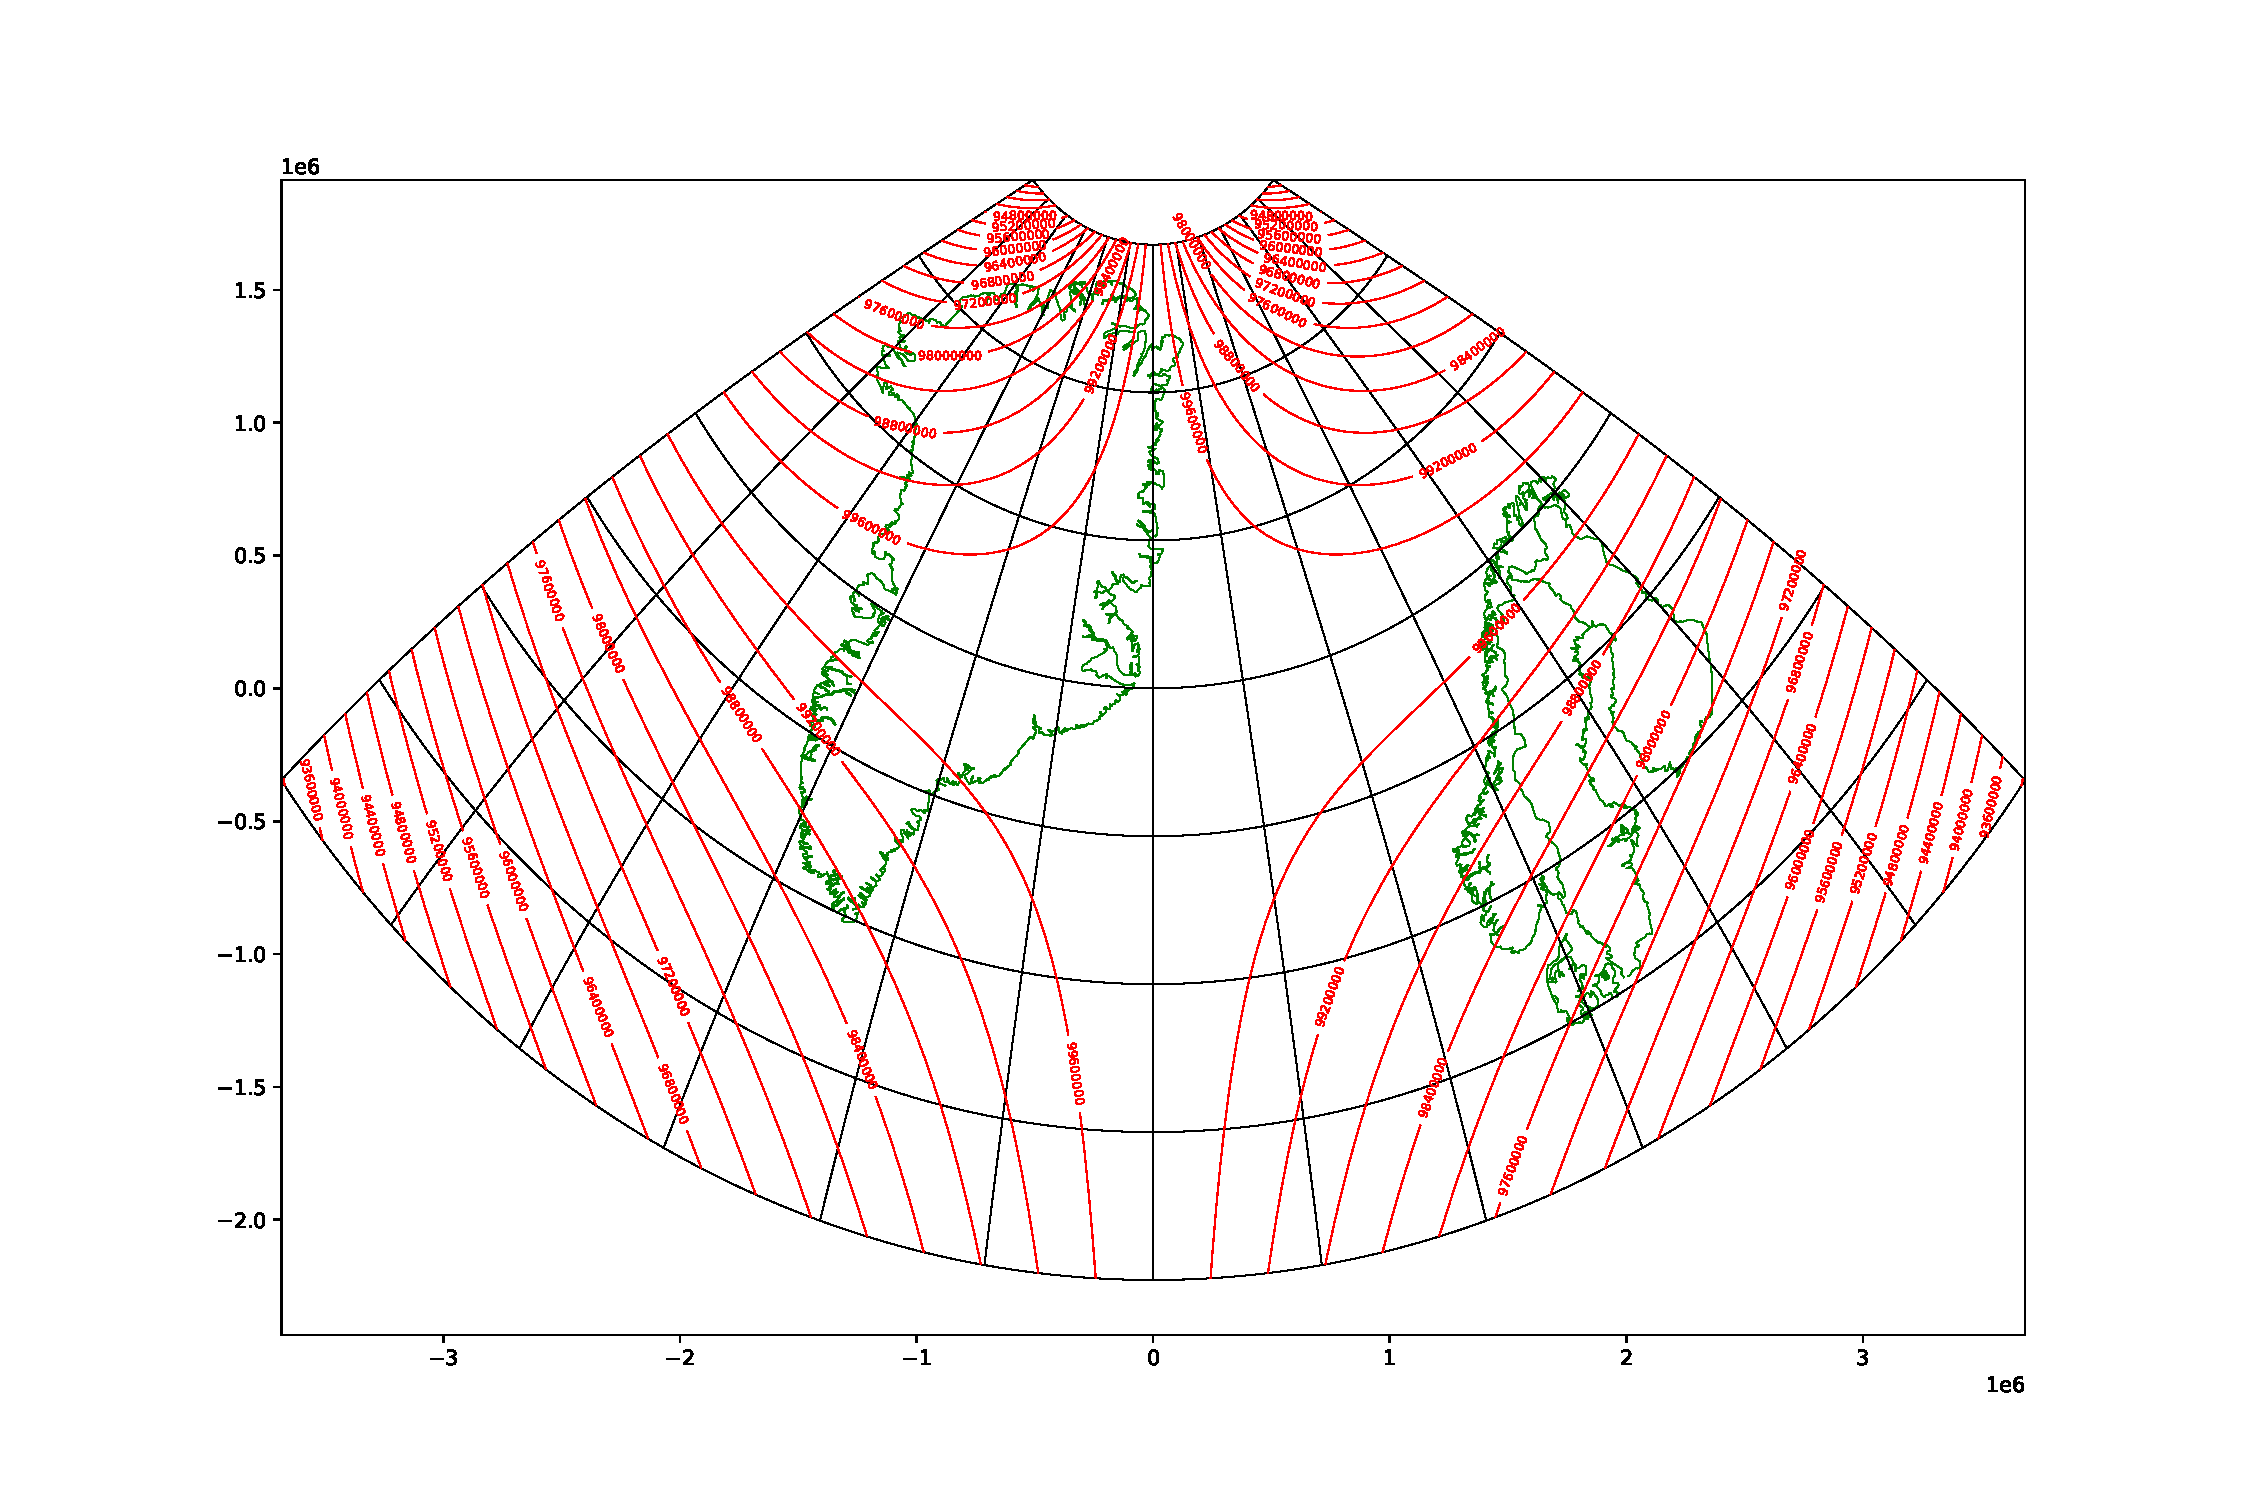
\includegraphics[width=1\textwidth]{img/bonne_100.pdf}
    \caption{Ekvideformáty měřítkového číla pro Bonneovo zobrazení}
\end{figure}

\begin{figure}[H]
    \centering
    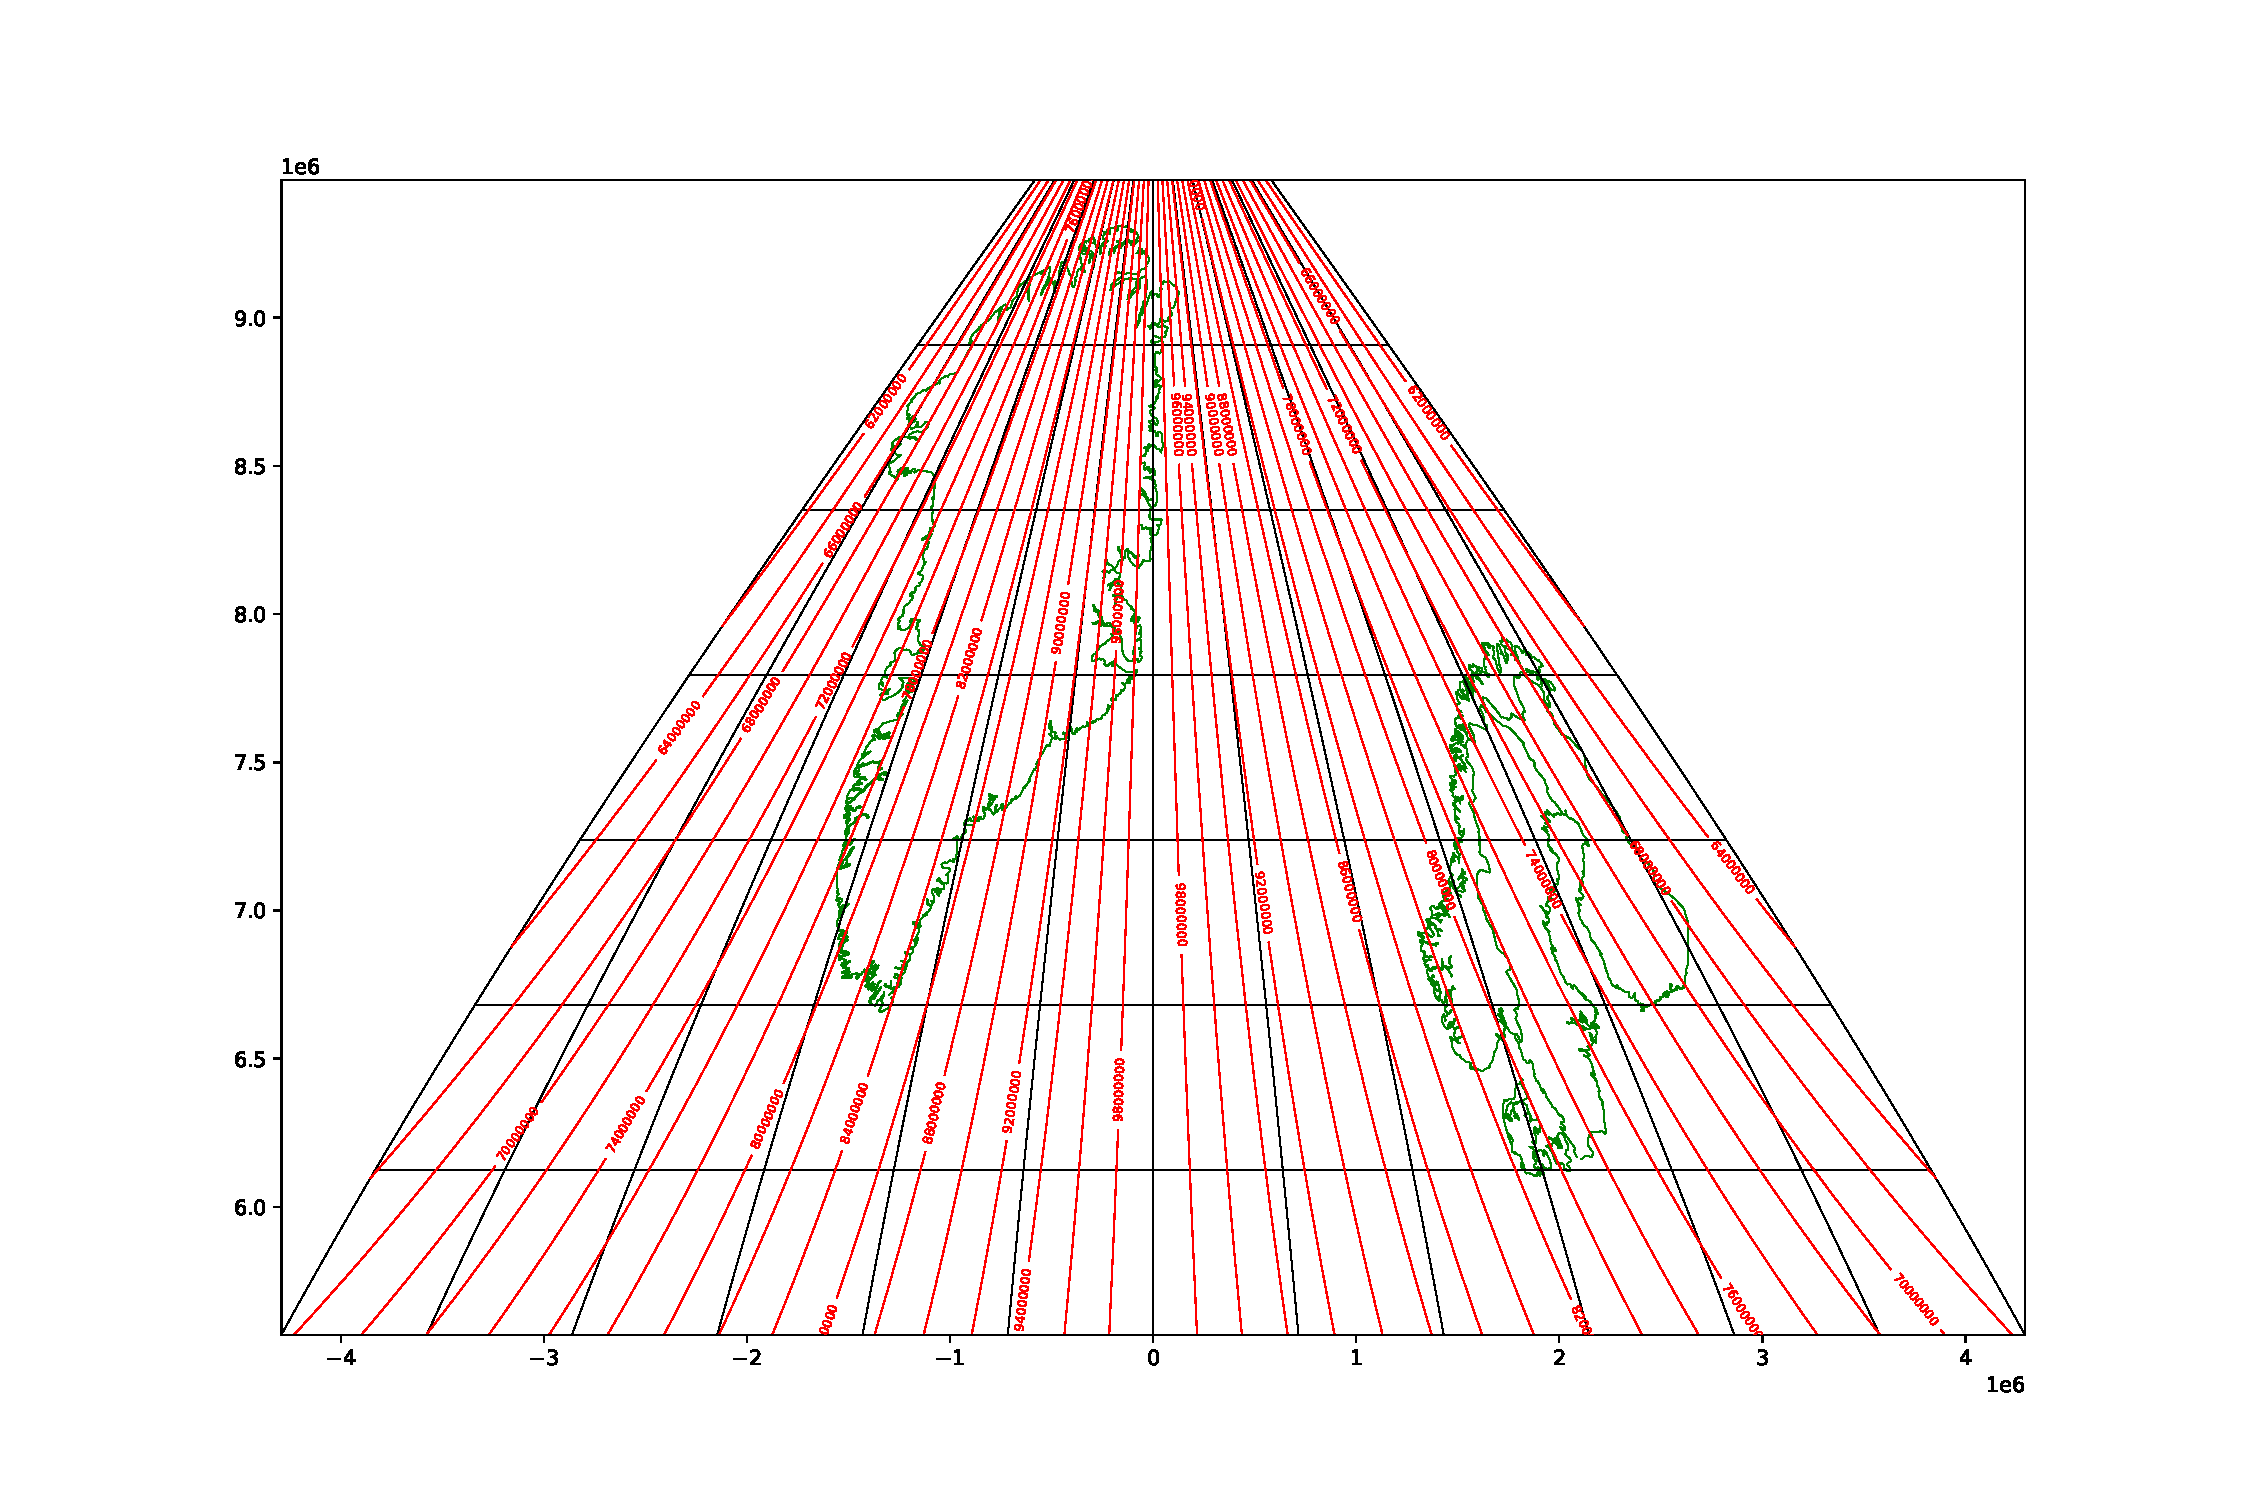
\includegraphics[width=1\textwidth]{img/sinu_100.pdf}
    \caption{Ekvideformáty měřítkového číla pro Mercator-Sansonovo zobrazení}
\end{figure}

\begin{figure}[H]
    \centering
    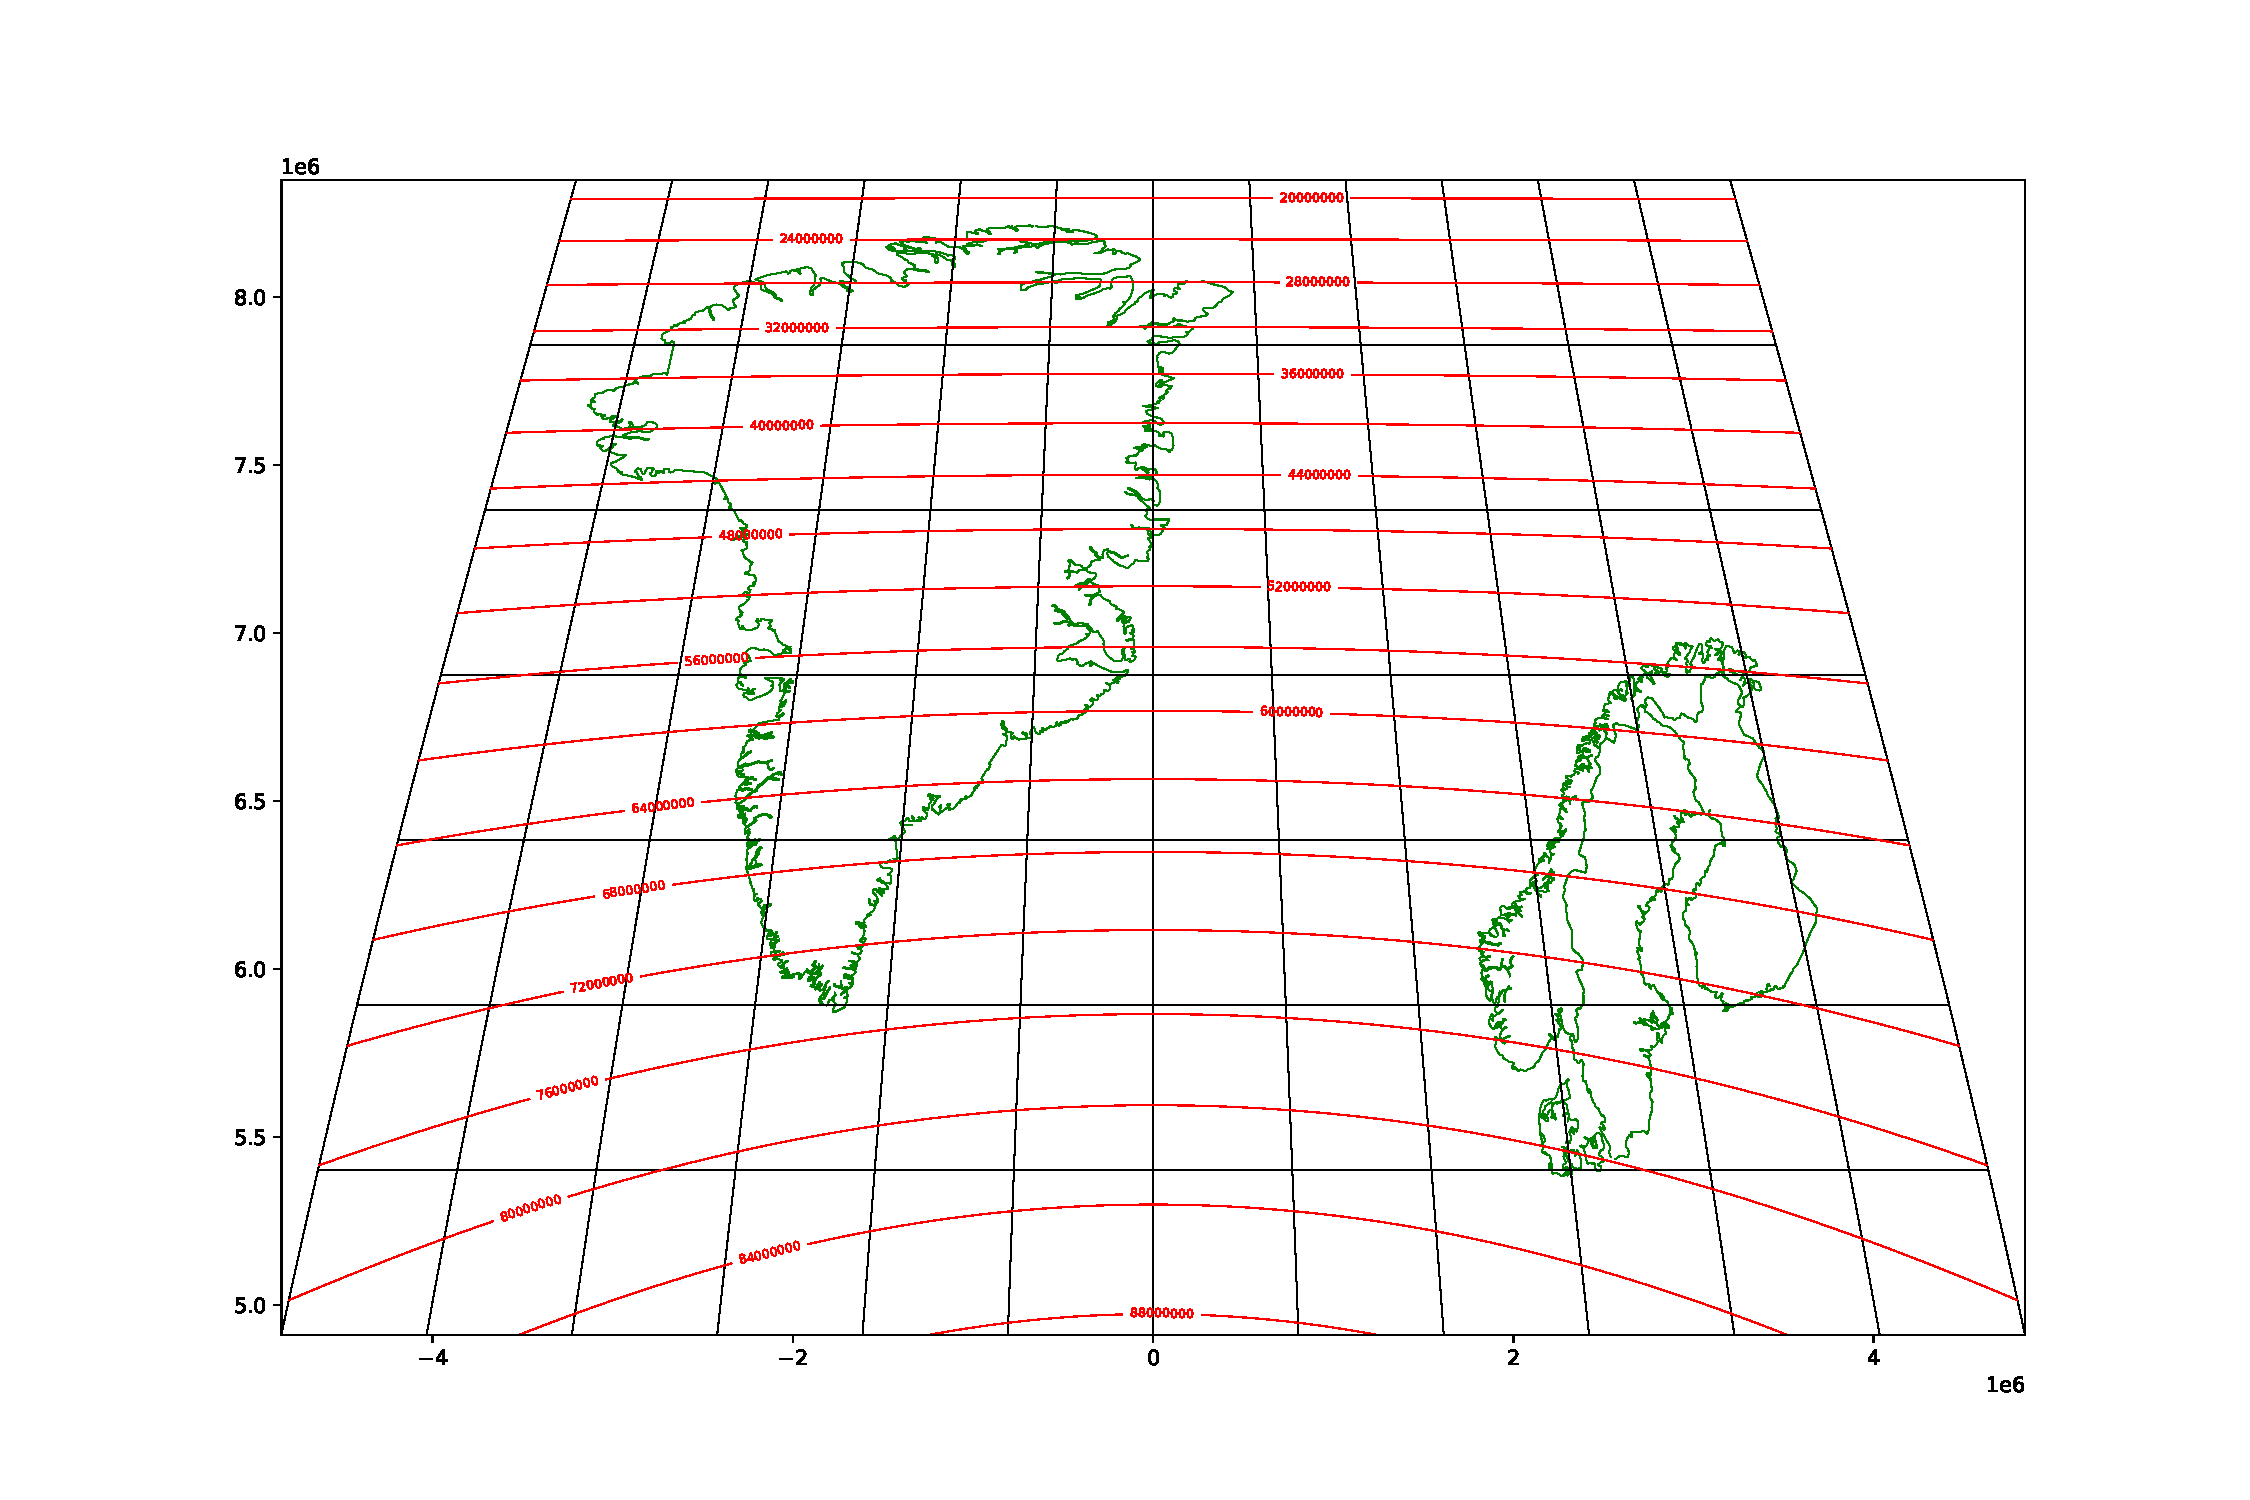
\includegraphics[width=1\textwidth]{img/eck5_100.pdf}
    \caption{Ekvideformáty měřítkového číla pro Eckertovo V. zobrazení}
\end{figure}

\begin{figure}[H]
    \centering
    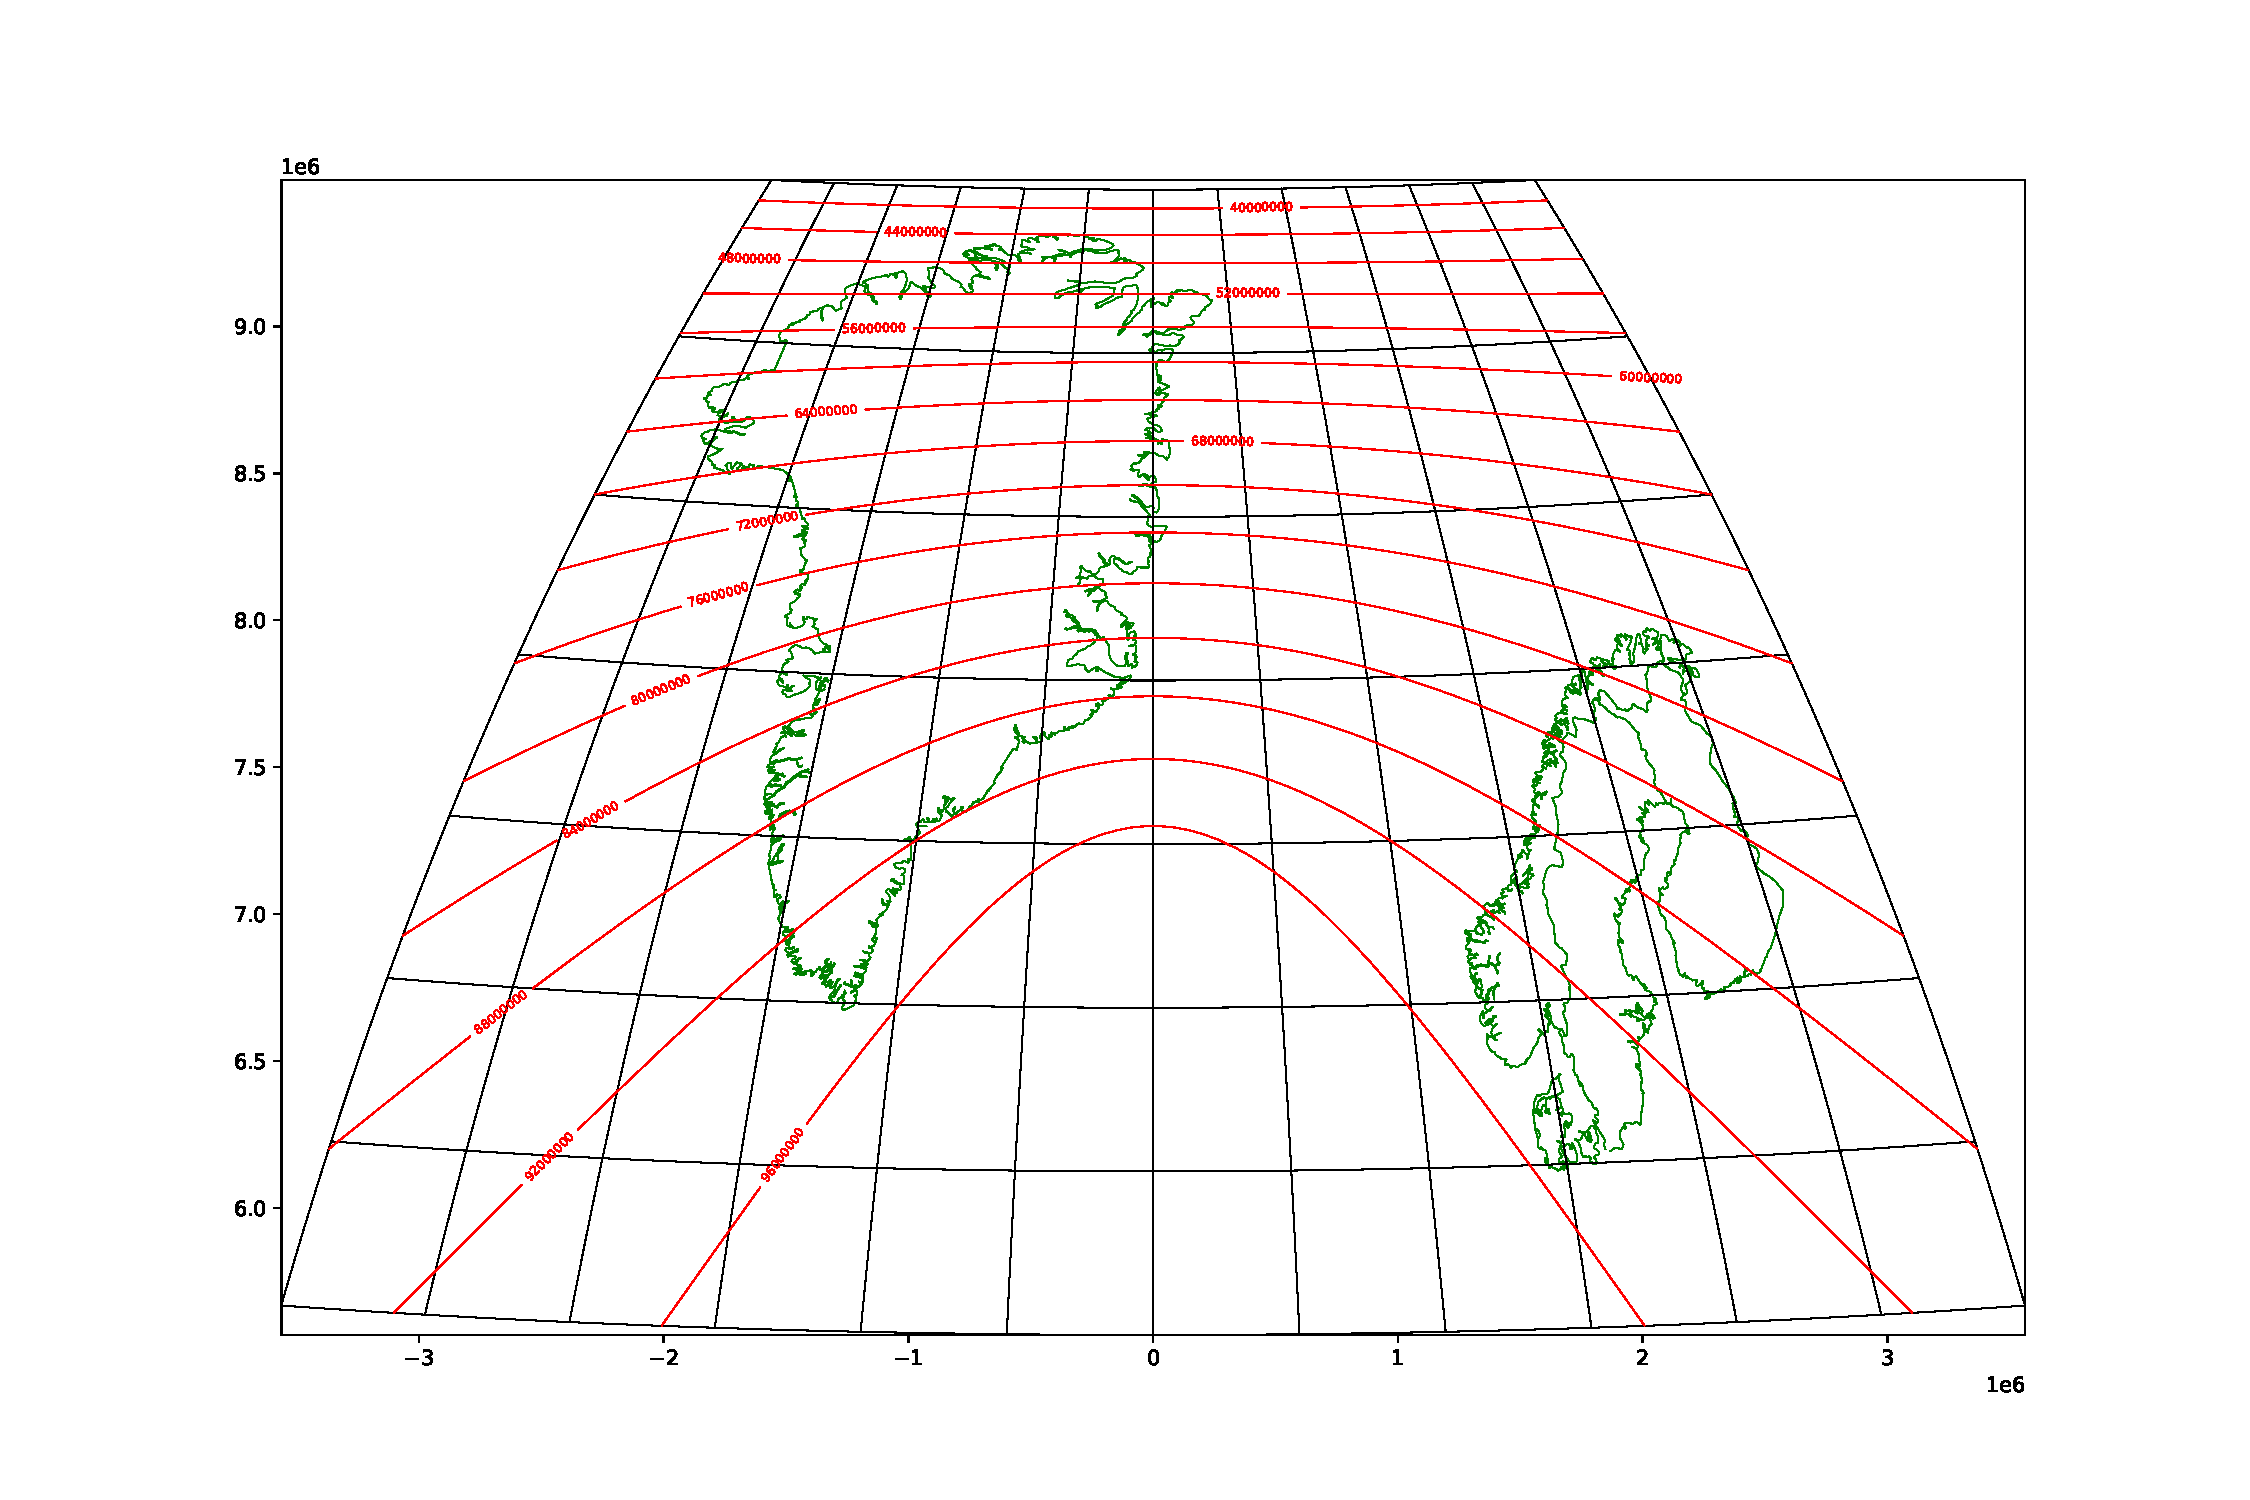
\includegraphics[width=1\textwidth]{img/wintri_100.pdf}
    \caption{Ekvideformáty měřítkového číla pro zobrazení Winkel-Tripel}
\end{figure}

\begin{figure}[H]
    \centering
    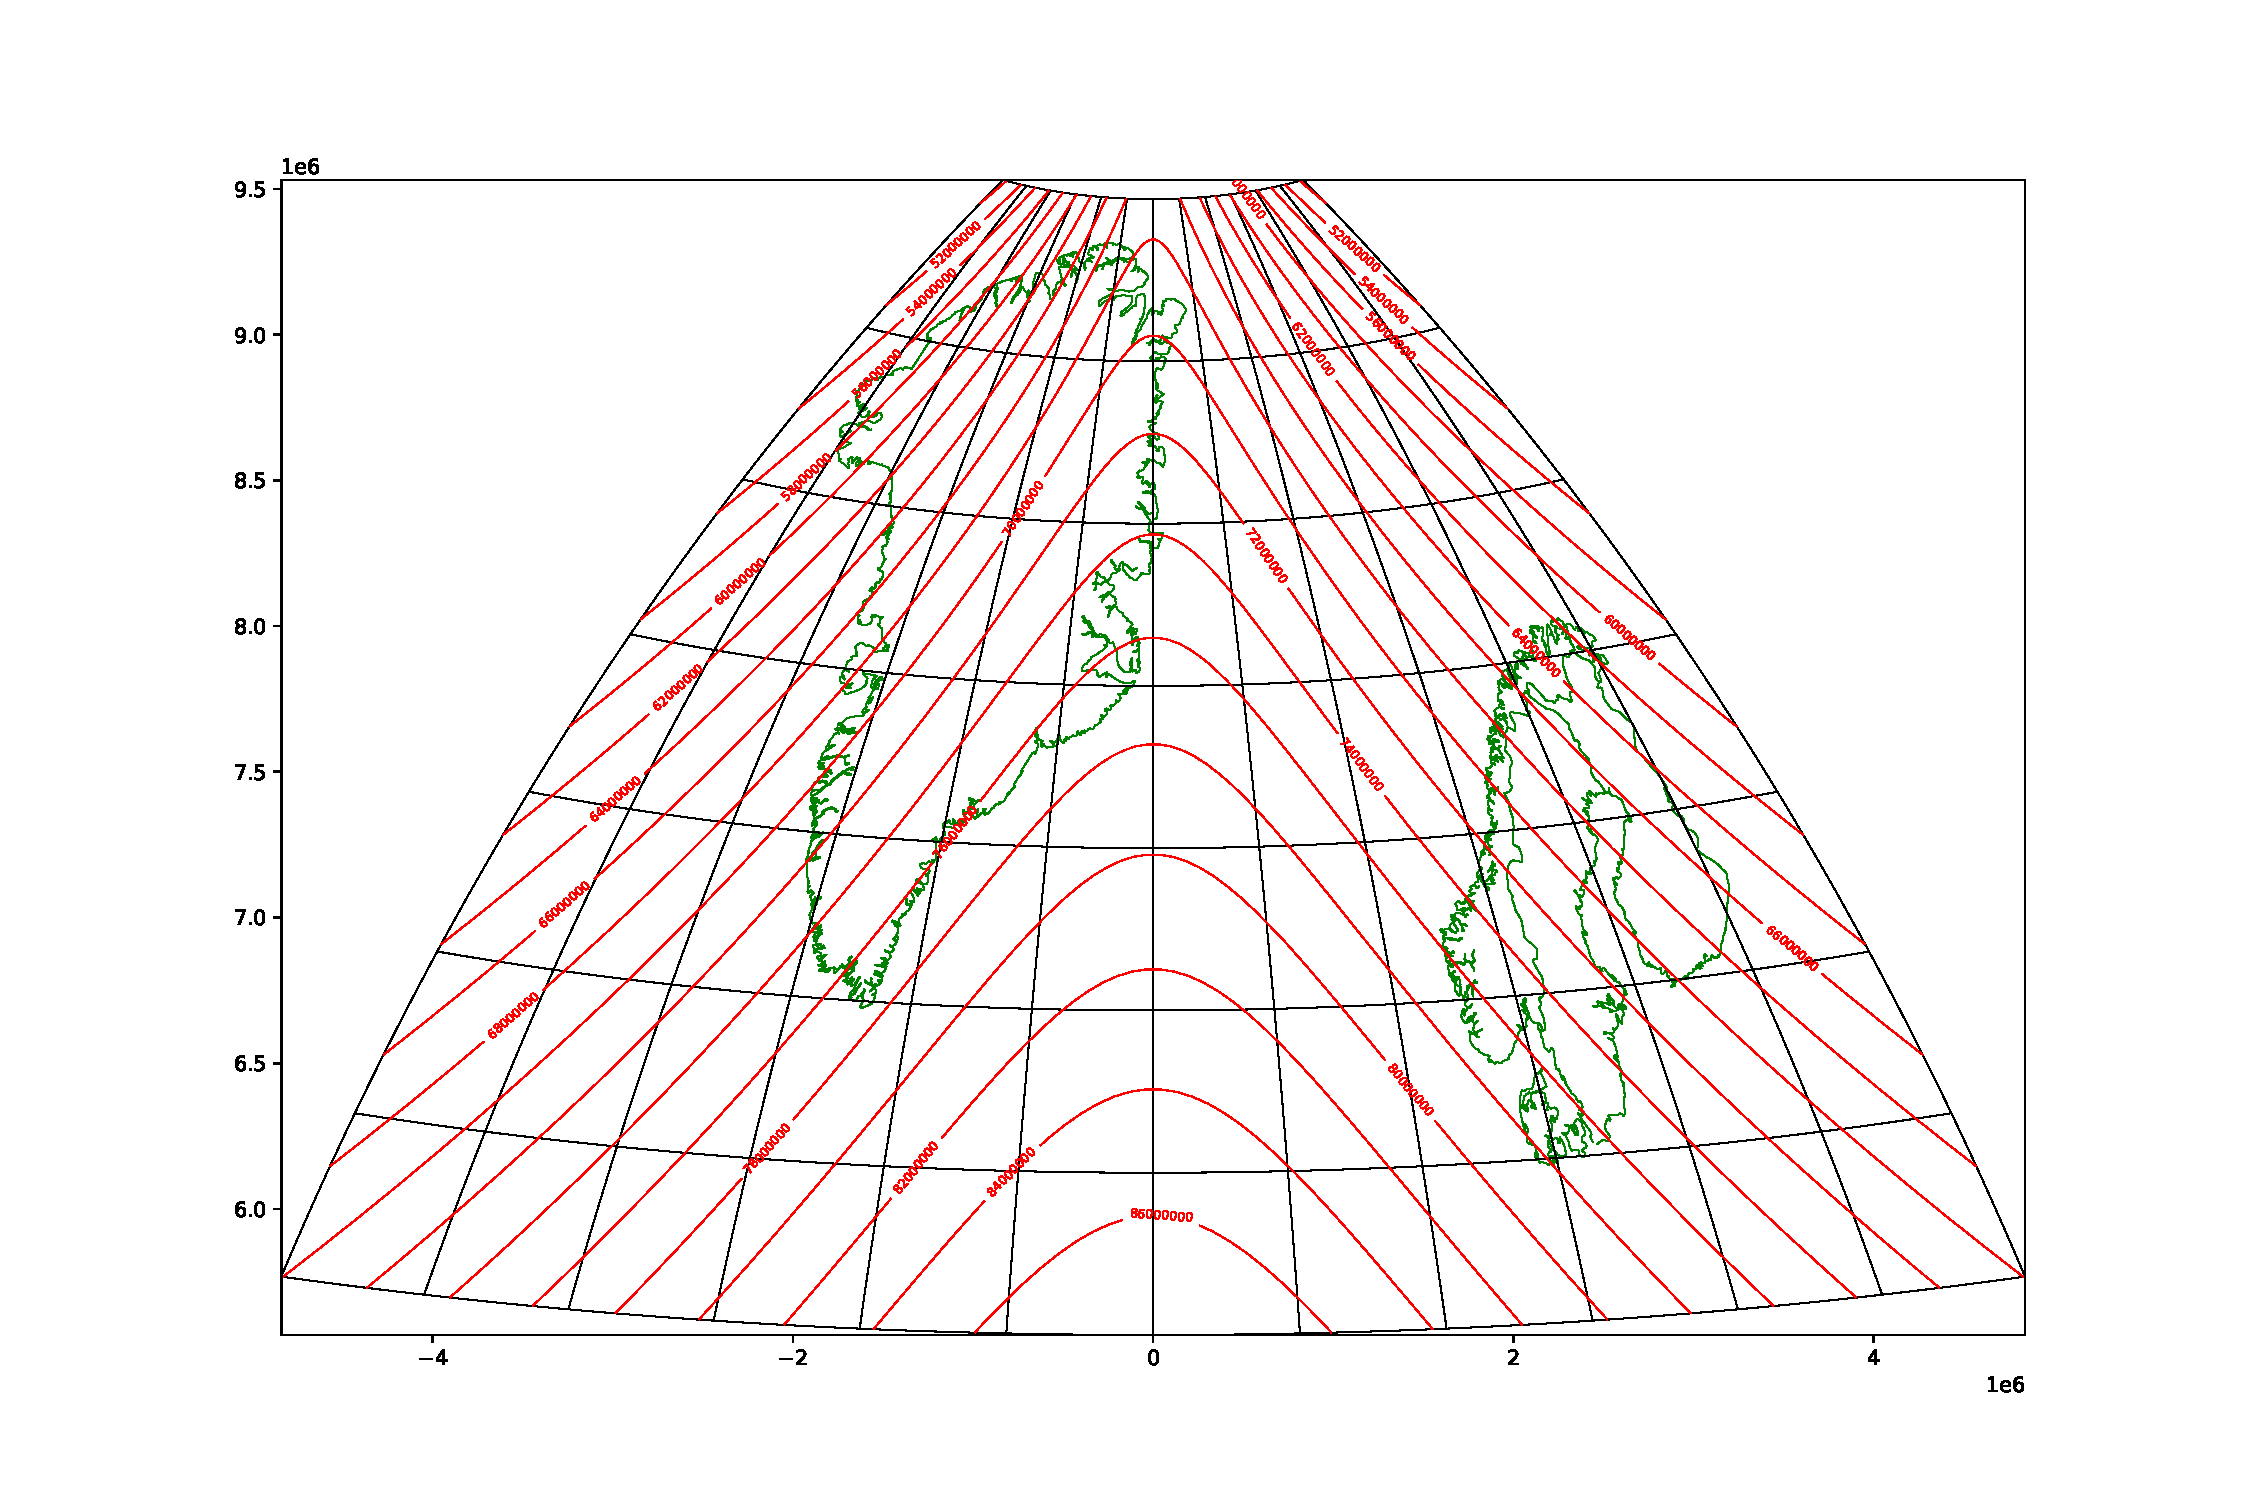
\includegraphics[width=1\textwidth]{img/aitoff_100.pdf}
    \caption{Ekvideformáty měřítkového číla pro Hammer-Aitoffovo zobrazení}
\end{figure}

\begin{table}[H]
    \centering
    \resizebox{\textwidth}{!}{
    \begin{tabular}{|l|c|c|c|c|c|c|}
    \hline
    \textbf{Zobrazení} & \textbf{Airy (neváž.)} & \textbf{Airy (váž.)} & \textbf{Komplex. (neváž.)} & \textbf{Komplex. (váž.)} & \textbf{Úhly $< 50^\circ$} & \textbf{Měřítko $< 50\,\%$} \\ \hline
    Bonneovo & 0.0005 & 0.0005 & 0.0492 & 0.0523 & 100.00\,\% & 100.00\,\% \\ \hline
    Mercator-Sansonovo & 0.0801 & 0.0749 & 0.9037 & 0.8684 & 95.16\,\% & 87.16\,\% \\ \hline
    Eckertovo V. & 0.9991 & 0.4298 & 1.8830 & 1.2867 & 70.98\,\% & 41.78\,\% \\ \hline
    Winkel-Tripel & 0.1371 & 0.0602 & 0.6696 & 0.4938 & 96.90\,\% & 77.10\,\% \\ \hline
    Hammer-Aitoffovo & 0.1247 & 0.0972 & 0.9028 & 0.8010 & 98.46\,\% & 65.64\,\% \\ \hline
    \end{tabular}
    }
    \caption{Hodnoty globálních variačních kritérií a procentuální zastoupení zkreslení pro zvolené území}
\end{table}

\newpage
\section{Závěr}

Pro úlohu zhodnocení kartografických zobrazení za pomoci variačních kritérií bylo jako zájmové území vybráno č. 21 skandinávské státy, Grónsko. Z vypočtených hodnot, které jsou zobrazeny v Tabulce 1 je patrné, že nejlepším zobrazením vyšlo Bonneovo zobrazení, které dosahuje nejnižších hodnot u Airyho i komplexního variačního kritéria. Nejhůř vyšlo zobrazení Eckert V., které se jeví jako nevhodné pro zobrazení tohoto území. U Airyho neváženého kritéria dosahoval výsledek téměř 1 a změny měřítka pod 50 \% na $42\,\%$ zobrazovaného území. 
\vspace{3mm}

\noindent Kompenzační a ekvivalentní zobrazení určená pro globální mapy (Winkel-Tripel, Hammer-Aitoffovo, Mercator-Sansonovo) se jeví jako vhodná volba díky jejich kompenzačním schopnostem, avšak pro zobrazení území, které je vzdálené od rovníku nepředstavují ideální volbu.
\vspace{3mm}

\noindent Nejlepším kritériem pro hodnocení zobrazení vyšla vážená varianta komplexního kritéria, která kombinuje hodnocení délkových i úhlových zkreslení a díky vážení zeměpisnou šířkou eliminuje drobné výkyvy na okrajích sítě.

\newpage
\section{Seznam literatury}
\vspace{3mm}

BAYER, T. (2026): \textit{Hodnocení zobrazení dle variačních kritérií (návod na cvičení)}. Výukový materiál pro předmět Matematická kartografie, Katedra aplikované geoinformatiky a kartografie, Přírodovědecká fakulta UK [cit. 5.6.2026].

\end{document}
